\chapter{ Констукторский раздел}
\label{cha:design}

Ниже представлены схемы алгоритмов -- Дамерау - Левенштейна и двух реализаций Левенштейна(рекурсивный и обычный).

\section{ Разработка алгоритмов}
\subsection{ Расстояние Левенштейна(обычный)}
На рисунке \ref{fig:default} представлена блок схема алгоритма Левенштейна.

\begin{figure}[ht!]
    \centering{
        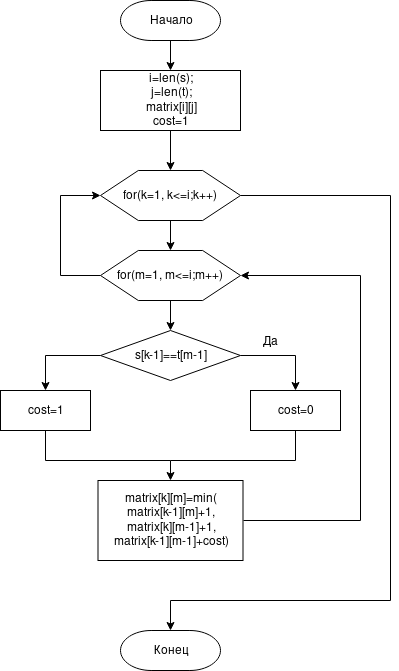
\includegraphics[width=0.4\textwidth]{img/levenstein.png}
        \caption{ Представлена схема алгоритма нахождения расстояния Левенштейна для матричной реализации}
        \label{fig:default}
    }
\end{figure}

\subsection{ Расстояние Дамерау -- Левенштейна}
На рисунке \ref{fig:damerau} представлена блок схема алгоритма Дамерау -- Левенштейна.

\begin{figure}[ht!]
	\centering{
        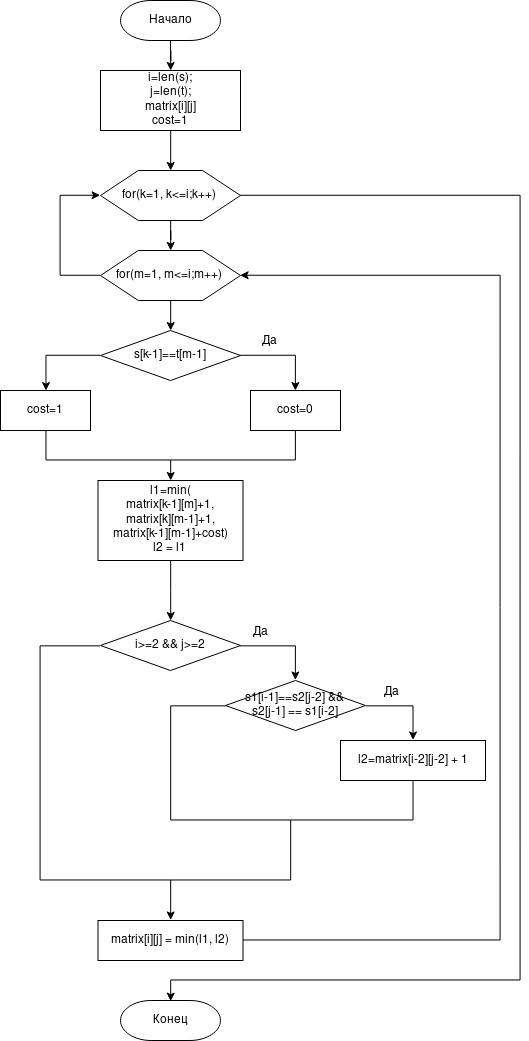
\includegraphics[width=0.4\textwidth]{img/damerau_levenstein.png}
        \caption{Представлена схема алгоритма нахождения расстояния Дамерау -- Левенштейна для матричной реализации}
        \label{fig:damerau}
    }
\end{figure}

\subsection{ Расстояние Левенштейна(рекурсивный)}
На рисунке \ref{fig:recursive} представлена блок схема рекурсивного алгоритма Левенштейна, в реализации которого используется функция \textit{int match(char c, char d)}, которая возвращает 0, если символы \textit{c} и \textit{d} совпадают, иначе 1. 

\begin{figure}[ht!]
	\centering{
        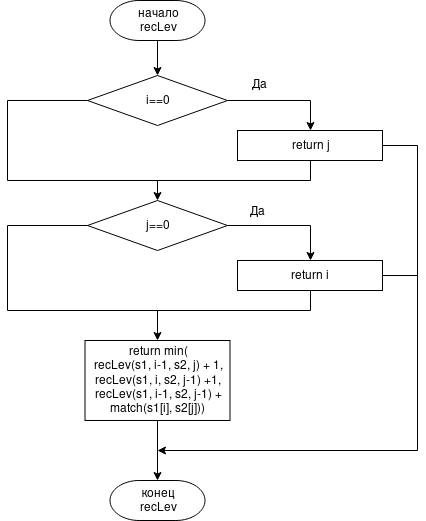
\includegraphics[width=0.4\textwidth]{img/recursive_levenstein.png}
        \caption{Представлена схема алгоритма нахождения расстояния Левенштайна для рекурсивной реализации}
        \label{fig:recursive}
    }
\end{figure}

 
